\section{Experimental setup}\label{experimentalSetup}

We now provide the main hardware and software specifications of the experimental setup used in our TPC-DS benchmark runs.

\subsection{Hardware configuration}\label{hardwareConfiguration}

Both, AWS EMR and Databricks UAP (concerning its AWS-based platform) run on the Amazon Elastic Compute Cloud (EC2). In order to best match the needs of particular customers and applications, EC2 offers a variety of instance types that optimize specific computational resources; concretely, memory, storage, or processing power (through vCPUs and GPUs). These in addition to general-purpose instances. Given the IO caching capabilities of Databricks, we opt for storage-optimized instances that incorporate an NVMe SSD, the i3.2xlarge type specifically. We use these instances for both systems and all of the experiments we present in this report. Furthermore, we fix the size of the clusters used in our experiments at 8 worker nodes and 1 master node. Table \ref{table:hardwareConf} summarizes the hardware configuration of the nodes we employ.

\begin{table}
  \centering
	\begin{tabular}{|l|l|l|l|}
	  \hline
		\textbf{Model} & \textbf{vCPUs} & \textbf{Memory} & \textbf{Local storage} \\ \hline
		i3.2xlarge & \makecell[l]{8 (2.3 GHz Intel \\ Xeon E5 2686 v4)} & 61 GiB & \makecell[l]{1 x 1,900 \\ GB NVMe SSD} \\ \hline
	\end{tabular}
	\caption{Hardware configuration.}
	\label{table:hardwareConf}
\end{table}

\subsection{Software configuration}

Next, we present the software configuration of the deployments of Databricks and EMR Presto employed in the experiments associated with our reference results.

\subsubsection{Databricks configuration}

The Databricks cluster creation GUI gives the user the alternative to choose among various versions of the Databricks runtime, subject to a deprecation schedule. A runtime version is in turn associated with a specific version of Apache Spark and the Scala programming language. In our case, we opted for the most recent production release of the runtime, namely version 5.3 with Spark 2.4 and Scala 2.11.

In addition to the Databricks runtime and its associated components, two configuration parameters for Spark were required for the correct execution of the benchmark. These are first, a high value for the broadcast timeout, to allow slower response times under a high load, and second, enabling the cross-join operation used in some queries. We present in Table \ref{table:softwareConfDatabricks} a summary of the software configuration for Databricks.

\begin{table}
  \centering
	\begin{tabular}{|l|l|}
	  \hline
		\textbf{Versions} & \textbf{Spark configuration parameters} \\ \hline
		Runtime 5.3, Spark 2.4, Scala 2.11 & \makecell[l]{spark.sql.broadcastTimeout = 7200 \\ spark.sql.crossJoin.enabled true} \\ \hline
	\end{tabular}
	\caption{Software configuration.}
	\label{table:softwareConfDatabricks}
\end{table}

\subsubsection{EMR Presto configuration}

At the time of the creation of the cluster, AWS EMR enables the user to select among various releases of the EMR platform, and subsequently to include many data processing frameworks, whose specific versions are determined by the release version. We used the most recent release, emr-5.23.0, with Presto 0.215. Additional frameworks were included, but these have no influence on the experiments. Furthermore, AWS Glue was selected as the metastore for the TPC-DS database to be created.

Specific configurations were found to be necessary to enforce the desired compression format and to avoid execution errors; Table \ref{table:softwareConfPresto} provides them as part of the summary of the EMR Presto configuration.

\begin{table}
  \centering
	\begin{tabular}{|l|l|}
	  \hline
		\textbf{Versions} & \textbf{Presto configuration parameters} \\ \hline
		emr-5.23.0, Presto 0.215 & \makecell[l]{hive.allow-drop-table: true \\ hive.compression-codec: SNAPPY \\
		hive.s3-file-system-type: PRESTO \\ query.max-memory: 240GB} \\ \hline
	\end{tabular}
	\caption{EMR Presto configuration.}
	\label{table:softwareConfPresto}
\end{table}

Since Presto relies on a Hive metastore accessed through a Hive connector, the first 3 parameters are prefixed with Hive. Allowing dropping tables is necessary when these need to be overwritten. The compression format used is SNAPPY. The PRESTO file system type is required to avoid timeout errors when accessing data in AWS S3. Finally, some queries require large amounts of memory across the cluster, hence the high value for the maximum memory of a query.

It is important to note that additional Presto configuration parameters were required for the successful completion of some queries, which did not occur in the analogous case for Databricks. We discuss these additional configuration parameters in Section \ref{referenceResults} dealing with the reference results.

\subsection{System pricing}\label{systemPricing}

For both of the SUTs, pricing is based on the time the clusters are used and consists of the EC2 instances costs plus the software costs.

\subsubsection{Databricks pricing}

For the Databricks UAP, the software component of pricing depends primarily on the type of cluster instantiated. From most to least expensive these are: Data Analytics, Data Engineering, and Data Engineering Light. The first supports notebooks and the full functionality of the workspace. The second is aimed at batch applications and comes with an optimized runtime, while the third also applies to batch applications but without the runtime optimizations. For the reference results, we opted for the second alternative. Additional costs are incurred for enterprise operational security capabilities, but these do not apply in our case. Adopting the i3.2xlarge EC2 instance types as stated earlier the full pricing is shown in Table \ref{table:systemCosts} alongside the EMR Presto costs, which we discuss next.

\subsubsection{EMR Presto pricing}

The pricing model for AWS EMR is simpler, consisting again of the EC2 instances and the software costs. The software costs do not vary depending on the data processing frameworks installed. An additional consideration is AWS Glue, which is serverless but has separate charges above the free tier. Given that the free tier covers storing up to a million objects, we will ignore such costs. The total price for EMR Presto is compared to that of Databricks in Table \ref{table:systemCosts}.

\begin{table}
  \centering
	\begin{tabular}{|l|l|l|l|}
	  \hline
		\textbf{System} & \textbf{\makecell[l]{EC2 cost per \\ node per hour}} & 
		\textbf{\makecell[l]{Software cost per \\ node per hour}} & 
		\textbf{\makecell[l]{Total cost per \\ node per hour}} \\ \hline
		\makecell[l]{Databricks (Data \\ Engineering)} & \$0.624 & \$0.30 & \$0.924 \\ \hline
	\end{tabular}
	\caption{System costs.}
	\label{table:systemCosts}
\end{table}

\subsection{Preliminary experiments}\label{preliminaryExperiments}

We performed a series of initial experiments to determine the computational resources needed to evaluate the TPC-DS Benchmark effectively and in a reasonable time. For this purpose, we ran the full benchmark on a cluster consisting of 4 worker nodes and one master node, using the hardware configuration specified in Section \ref{hardwareConfiguration} (Table \ref{table:hardwareConf}), thus half the number of worker nodes as the experiments in the rest of this report. We will explain shortly the reason for doubling the number of worker nodes. We also used the default configuration for both Databricks and EMR Presto, and the original TPC-DS queries except for minor modifications for compatibility (in later experiments we modified two queries for EMR Presto as we describe in Section \ref{referenceResultsPowerTest}). Finally, the tables were stored in Databricks File System (DBFS), which is supported by S3, thus potentially similar to our S3 storage setup for our other experiments.

This initial experiment proved successful for Databricks, and we present a summary of the results in Figure 17. The total execution time adds up to 21.91 hours, which incidentally is about 2.28 times as much as the time required to evaluate the benchmark in our reference configuration detailed in Section \ref{referenceResults}, which as noted used 8 worker nodes instead of 4. Therefore, although two queries were different as noted above, we observe a good elasticity in the use of resources for Databricks.

\begin{figure*}
		\centering
		\begin{tabular}{|l|l|l|}
		\hline 
				\scalebox{0.25}{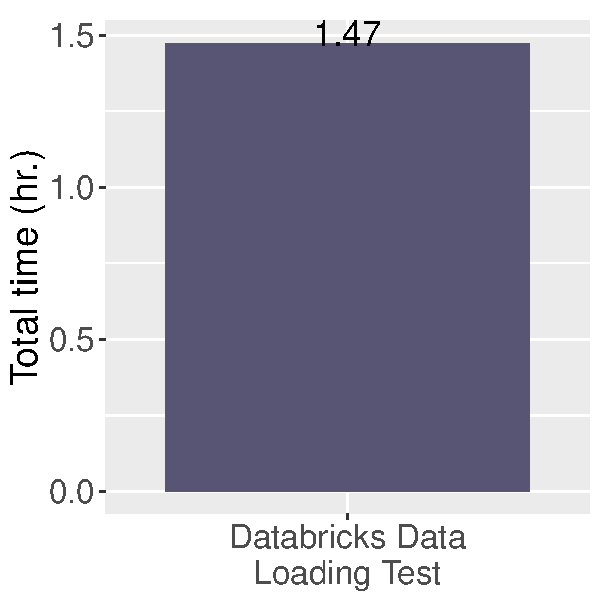
\includegraphics[width=7.0in]{imgs/experimentalSetup/load_totalHrTimeBarChart.pdf}}
				&
				\scalebox{0.25}{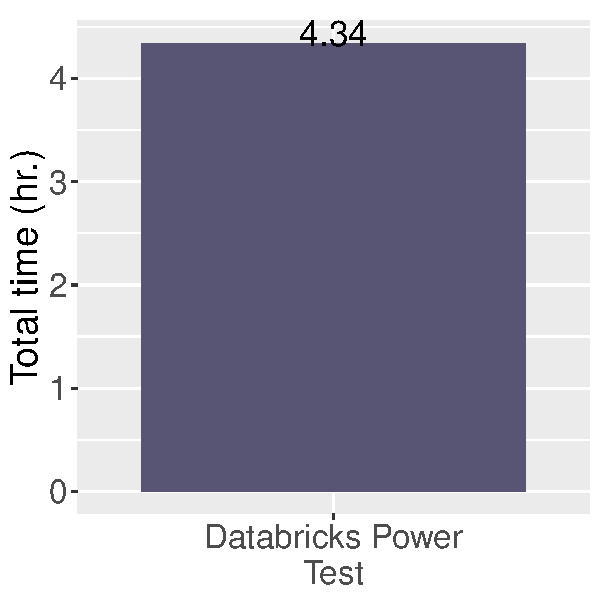
\includegraphics[width=7.0in]{imgs/experimentalSetup/power_totalHrTimeBarChart.pdf}}
        &
        \scalebox{0.25}{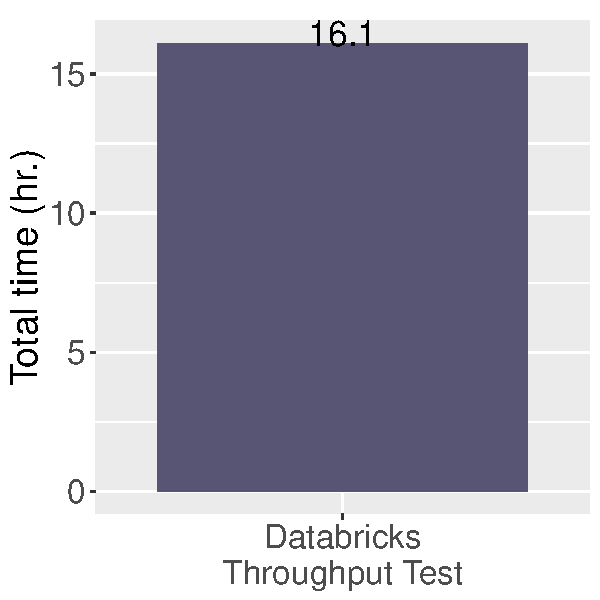
\includegraphics[width=7.0in]{imgs/experimentalSetup/tput_totalHrTimeBarChart.pdf}} \\
				\hline
		\end{tabular}
		\caption{Preliminary experimental results with Databricks.}
		\label{fig:preliminaryResults}
\end{figure*}

In the case of EMR Presto, many queries failed due to memory related errors, either the memory available within a particular node was insufficient or the memory allocated in total to a query across the cluster was insufficient. For this reason, we doubled the number of worker nodes to 8, aiming to avoid at least the first type of memory error. This, however, proved to be insufficient, so we needed to introduce the configuration modifications and query rewritings detailed in Section \ref{referenceResultsPowerTest}.



